% !TeX root = ../main.tex
% -*- coding: utf-8 -*-

\chapter{协同线性流形学习算法介绍}
\label{chpt:method}
协同线性流形学习(Collaborative Linear Manifold Learning,CLML)是一个基于流形学习做链接预测的算法。
该算法首先假设了数据空间是一个低维嵌入,利用辅助矩阵和目标矩阵分别学习到了两个流形,通过“两个流形具有一致性”这个假设定义出了带低秩约束的损失函数;
最后,算法使用随机梯度下降对模型进行优化。图\ref{method:fig:CLML}以药物-药物关联预测为例展示了算法的主要流程,本章将分小节介绍该算法的各个部分。

\begin{figure} 
  \centering
  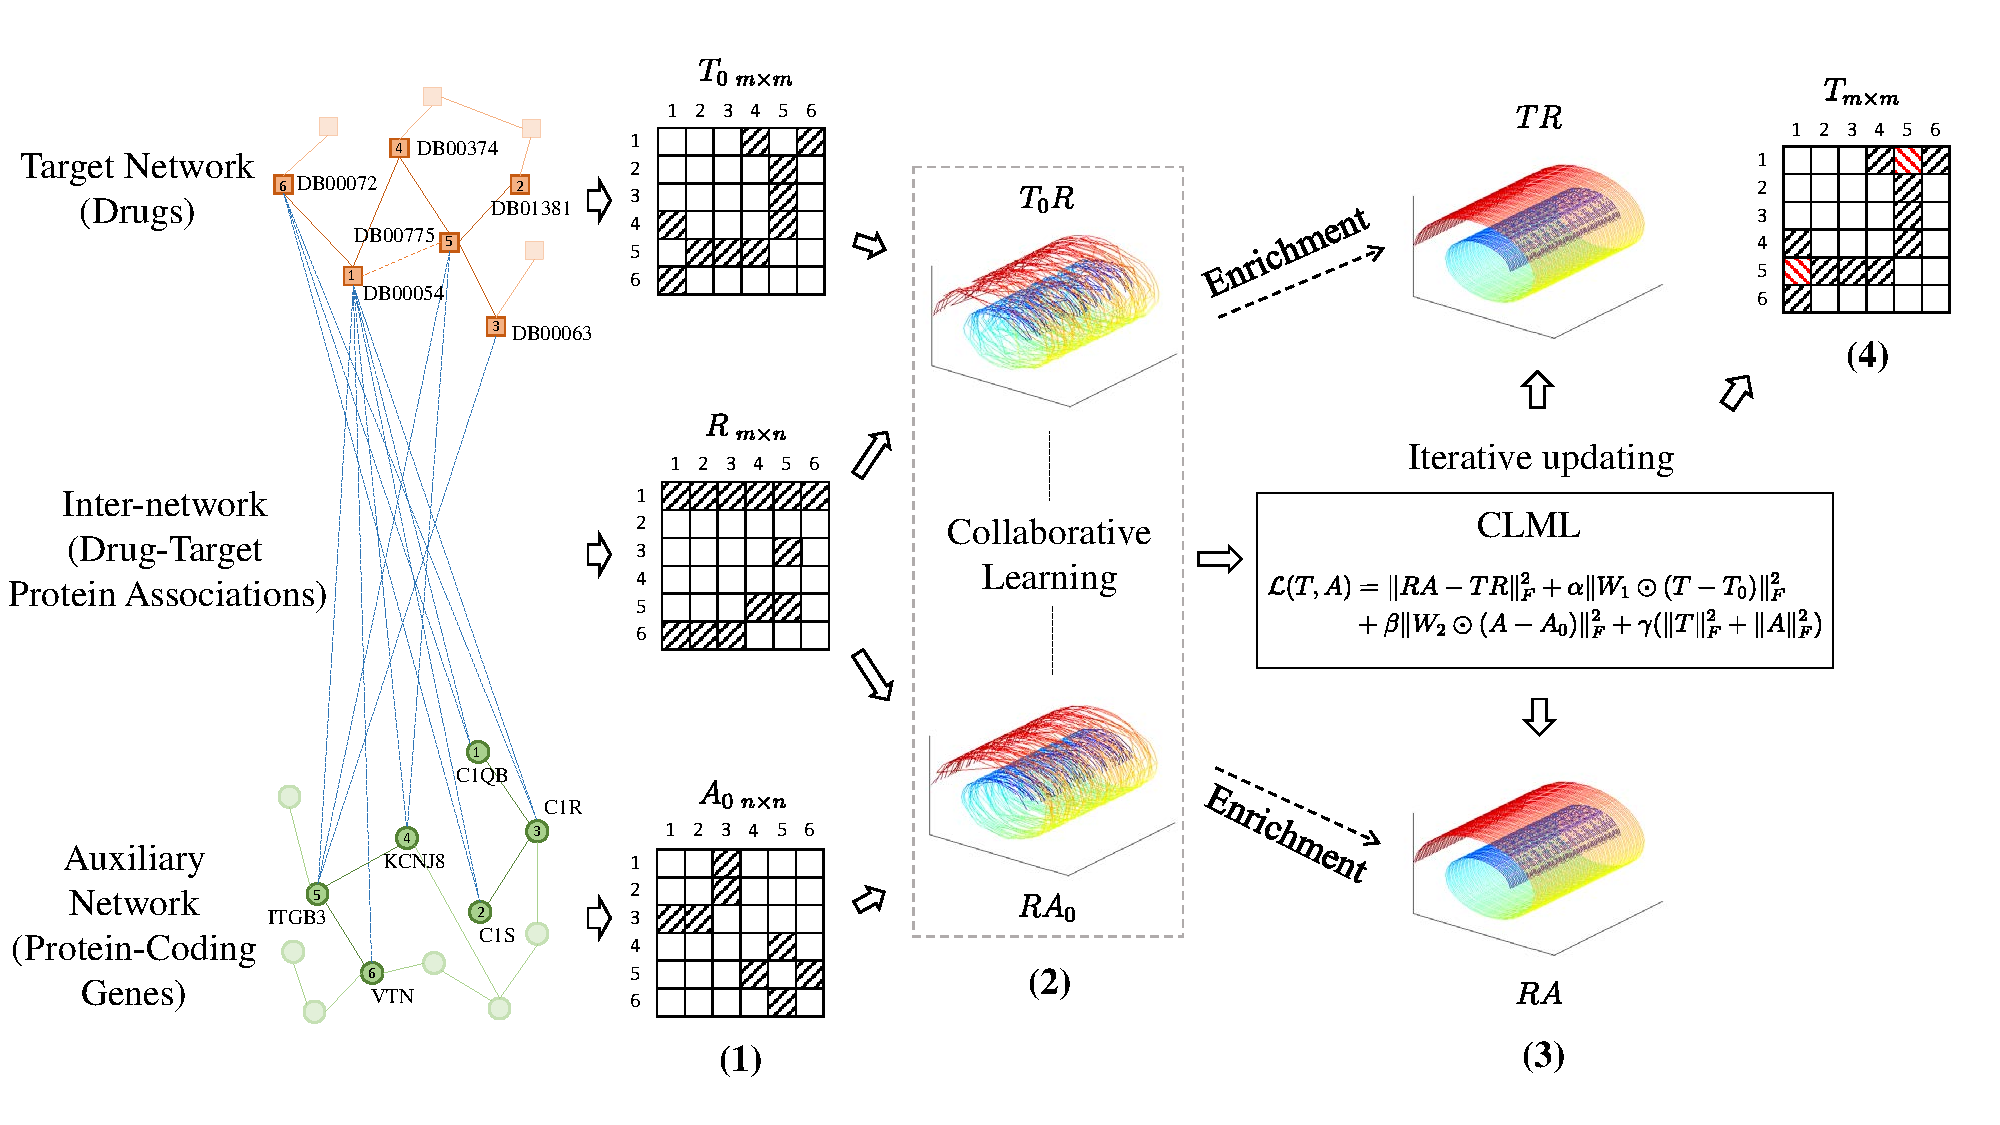
\includegraphics[width=0.99\linewidth]{CLML.pdf}
  \caption{CLML算法主要流程}
  \label{method:fig:CLML}
\end{figure} 


\section{符号表示}
\label{method:sec:notations}

为了简化算法推导过程中对所用符号的解释并保持上下文符号一致性,本节总结了将要用到的所有重要符号并做了解释,各符号意义参见表\ref{method:table:notations}。
\zihaowu
\begin{center}
\tablecaption{各符号释义}
\begin{tabular}{ll} \hline
    符号 & 意义 \\ \hline
    $m$         & 目标矩阵的规模 \\
    $n$         & 辅助矩阵的规模 \\
    $D_{m*m}$   & 目标矩阵 \\
    $R_{m*n}$   & 网络间关联矩阵 \\
    $T_{n*n}$   & 辅助矩阵 \\
    $I_n$       & $n*n$的单位矩阵 \\
    $\Arrowvert{X}\Arrowvert_{F}$ & X的Frobenius范数 \\
    $\Arrowvert{X}\Arrowvert_{*}=\sum_{i}\sigma_i$ & $X$的核范数 \\
    $\sigma_i$  & 矩阵第i大的奇异值 \\
    $X\odot{Y}$ & $X$与$Y$的哈达玛积 \\
    $\langle{X},\ Y\rangle$ & X与Y的内积 \\ \hline
\end{tabular}
\label{method:table:notations}
\end{center}
\zihaoxiaosi

目标矩阵就是我们要对其预测的矩阵,辅助矩阵就是算法中引入的辅助信息对应的矩阵,网络间关联矩阵就是这两各矩阵间的关系。
如在DDI预测中,药物-药物关联矩阵就是目标矩阵,蛋白-蛋白关联矩阵就是辅助矩阵,药物-靶蛋白关联矩阵就是网络间关联矩阵。


\section{线性流形学习}
\subsection{先验约束}
\label{method:subsec:prior}
流形学习(manifold learning)是一类借鉴了拓扑流形概念的降维方法,它把数据看作是一个嵌入在高维空间中的低维结构。
因此,虽然数据维度可能很高或在高维空间分布很复杂,但在局部却仍具有欧式空间的性质,可利用欧式距离重新进行距离测算,
在局部建立降维映射关系来将数据映射到低维空间中。


局部线性嵌入(Locally Linear Embedding,LLE)是流形学习的一个著名算法。
LLE假设,在高维空间中的任意一个点,在局部范围内(它的k近邻点)近似位于一个超平面上,
所以该样本点可以通过其k近邻点的线性组合重构出来,即空间中的一点满足式(\ref{method:formula:self_repre})。


\begin{equation}
    \hat{X_i}=\sum_{j\in\phi(i)}\omega_{ij}X_j \label{method:formula:self_repre}
\end{equation}

其中,$\phi(i)$表示点i的k近邻点集合,$\omega_{ij}$为线性重构时每个点的权重系数,为$\omega_{ij}$找到合适的值后便可令每个点都由其近邻点线性表出。


LLE算法的不足之处在于,当数据过于稀疏时容易产生“断路”,即某些点无法找到k个足够近的近邻点。
而在稀疏子空间聚类(Sparsity Subspace Clustering,SSC)算法将空间内的每个点都由该点所在的子簇内的所有点共同表出\cite{elhamifar2013sparse}。
因此,在考虑了数据稀疏的问题后,CLML结合了LLE和SSC算法的思想,将线性重构过程中使用的数据扩展到了全局范围内,
即每个点均使用空间内其余所有点来线性表出而不再仅使用其k近邻点,即使其余点并未与该点直接相连,如图\ref{method:fig:global_manifold}所示。

\begin{figure}
    \centering
    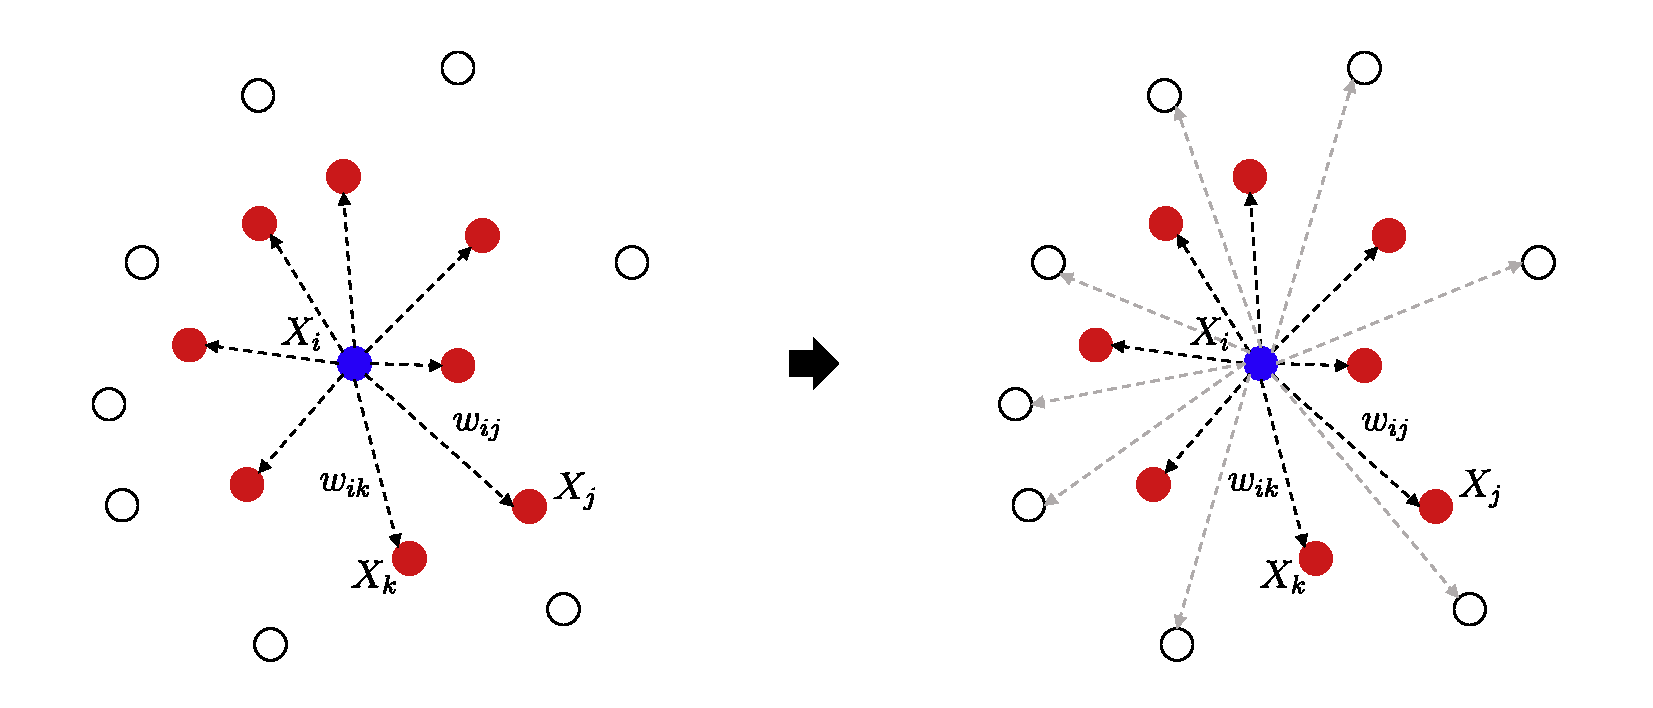
\includegraphics[width=0.9\linewidth]{global_manifold.pdf}
    \caption{将构建流形使用的点扩张至全局范围内}
    \label{method:fig:global_manifold}
\end{figure}

因此我们得到了式(\ref{method:formula:constraint})中的对先验数据的约束,其中$W_{ij}$便是为了控制与点直接相连和不直接相连的点在线性重构时的权重。
$W_{ij}$的取值如式(\ref{method:formula:weight})所示,里面的$\mu$是一个介于[0, 1]内的可调节的参数,
为了让与节点直接相连的点在重构时的权重更大,与节点距离较远的点权重更小,通常令$\mu\geq0.5$;
$\rho$是一个足够大的数来保证矩阵对角线元素接近0,这使得每个点只能由其余点来表示(而不是用自己表示)。

\begin{equation}
    f(D)=\sum^m_{i=1}\sum^m_{j=1}W_{ij}(D_{ij}-D_{0ij}) \label{method:formula:constraint}
\end{equation}


\begin{equation}
    W_{ij}=\begin{cases}
        \mu,& if\ \ D_{0ij} = 1 \\
        1 - \mu,& if\ \ D_{0ij} = 0 \\
        \rho,& if\ \ i = j
        \end{cases}
        \label{method:formula:weight}
\end{equation}


我们大费周章地将$D_0$矩阵中每个点都用空间中其余点表示的目的,就是为了用另一种方式构建出一个新的矩阵$D$,
使最终学习到的$D$和$D_0$的结构相近但二者又有所不同。
其中,$D$为了满足该约束所添加的新的链接就是我们对网络潜在链接的预测结果。

\subsection{重构线性流形}

在上一小节中我们得到了用$D$矩阵近似表示$D_0$所用的约束,接下来我们需要提出具体的损失函数,依靠损失函数我们才能最终学习到具体的$D$矩阵。


我们观察到,矩阵$D$、$R$的结构类似,也就是说使用$D$线性重构$R$矩阵后得到的结果$R_d=R*D$仍为$m*n$的矩阵且仍代表网络间的相互关系。
于是,我们利用这一特点对$R$和$R_d$的近似做了约束。为了防止过拟合,我们还加入了对矩阵$D$的正则化项,最终得到式(\ref{method:formula:simple_ver})。
\begin{align}
L(D)&=\sum_{i=1}^m\Arrowvert{R_i-\sum_{j\neq{i}} R_jD_{ij} }\Arrowvert^2 + 
\alpha\sum_{i=1}^m\sum_{j=1}^mW_{ij}(D_{ij}-D_{0ij})+\gamma\Arrowvert{D}\Arrowvert_F^2\nonumber \\
    &= \Arrowvert{R-RD}\Arrowvert_F^2+\alpha\Arrowvert{W}\odot(D-D_0)\Arrowvert_F^2+\gamma\Arrowvert{D}\Arrowvert_F^2
    \label{method:formula:simple_ver}
\end{align}

式中,$\alpha$和$\beta$为超参,分别控制先验数据的约束项和正则项对损失函数的影响。最终学习到的$D$矩阵中的每个元素将是一个在[0, 1]范围内的连续数值,
做预测时可再令$P=(\arrowvert{T^*}\arrowvert+\arrowvert{T^{*^T}}\arrowvert)/2)$即可得到一个对称矩阵$P$,
其中$P_{ij}$的值代表节点$i$和节点$j$产生链接的概率,$P_{ij}$越大则两点间越可能产生链接。


\subsection{低秩约束}

如果一个矩阵的秩远小于它的维数,则可称为其低秩矩阵。低秩也代表着矩阵行、列间的相关性很强,可以互相线性表出,
该特性可以很好的运用在特征分析或矩阵补全(如图像修复、链接预测等)上,而在\ref{method:subsec:prior}节中提到,算法需要让矩阵$D$中的每个点均由其余点线性表出,
因此可以通过引入低秩约束来更好地满足这一需求。为保持矩阵低秩,可对矩阵使用$L0$范数约束,但$L0$范数的优化是个NP难问题,
为此我们使用核范数来近似,也即令式(\ref{method:formula:simple_ver})中的F范数替换为$\Arrowvert{D}\Arrowvert_*^2$。


\section{协同学习}
\label{method:sec:collaborative}
在上一节中利用$R$和$R_d$的相似性已经可以对目标矩阵进行链接预测了。但实验发现,$R$矩阵往往较为稀疏,
仅利用$R$和$R_d$之间的相似性得到的预测结果并不好,且观察后发现$R$和$R_d$之间仅有50\%左右的相似性。


但注意到,辅助矩阵$T$和$R$同样具有相似的结构,使用$T$来重构$R$后得到的新的矩阵$R_t=T*R$同先前一样,都应和$R$矩阵近似,
因此可以很快推导出式(\ref{method:formula:reverse_ver})。
\begin{align}
L(T)&=\sum_{i=1}^m\Arrowvert{R_i-\sum_{j\neq{i}} T_{ij}R_j }\Arrowvert^2 
+\alpha\sum_{i=1}^m\sum_{j=1}^mW_{ij}(T_{ij}-T_{0ij})+\gamma\Arrowvert{T}\Arrowvert_*^2 \nonumber \\
    &=\Arrowvert{R-TR}\Arrowvert_F^2+\alpha\Arrowvert{W}\odot(T-T_0)\Arrowvert_F^2+\gamma\Arrowvert{T}\Arrowvert_*^2
    \label{method:formula:reverse_ver}
\end{align}


值得注意的是,在式(\ref{method:formula:simple_ver})和式(\ref{method:formula:reverse_ver})中的重构部分使用的是同一个R矩阵,
即算法对$R_d$与$R_t$都做了与$R$结构近似的约束,区别仅在于在重构时$R_d$和$R_t$使用的是不同的先验数据。
既然$R_d$和$R_t$都与矩阵$R$近似,那么理论上$R_d$和$R_t$的结构也应具有一致性,即$R_d \approx R_t$。基于此,我们提出了如式(\ref{method:formula:dual_ver})所示的协同学习算法的损失函数,
式中$W_1$、$W_2$的取值和作用与式(\ref{method:formula:simple_ver}), 式(\ref{method:formula:reverse_ver})相同,$\alpha$、$\beta$仍为超参。
\begin{align}
L(D,\ T)=&\Arrowvert{RD-TR}\Arrowvert_F^2+\alpha\Arrowvert{W_1}\odot(T-T_0)\Arrowvert_F^2 \nonumber\\
        &+\beta\Arrowvert{W_2}\odot(D-D_0)\Arrowvert_F^2+ \gamma(\Arrowvert{T}\Arrowvert_*^2+\Arrowvert{D}\Arrowvert_*^2)
        \label{method:formula:dual_ver}
\end{align}

通过协同学习的方式我们可以克服由于$R$矩阵数据稀疏导致重构后的结构不完整,两矩阵差异较大(仅50\%的相似度)的问题。
实验发现,使用协同学习后$R_d$和$R_y$能达到接近98\%的相似度,这足以说明引入协同学习的必要性和算法的实际效果。

\section{本章小结}
本章首先介绍了一个基于线性流形学习的链接预测算法,算法利用原始数据构建了一个与关联矩阵结构类似的流形结构,利用二者结构的相似性对网络进行了链接预测。
但受到数据稀疏性的影响,重构后的流形结构并不完整,实验后的效果难以达到预期。
为此,我们又引入了辅助信息,利用辅助信息构建出了另一个与关联矩阵结构近似的流形结构。
利用双流形的近似性,我们使用了协同学习来克服数据稀疏的问题,使最终实验效果达到了预期。
